\chapter{Informationsbeschaffung}
\label{chap:Informationsbeschaffung}
Dieses Kapitel bietet fundamentale physikalische Gegebenheiten, sowie die relevanten Informationen über \ac{PIR} und verwendete 



\section{Physikalische Grundlagen}

Die Physikalischen Grundlagen 



\section{verwendete Sensorik}


\begin{figure}[H]
	\centering
	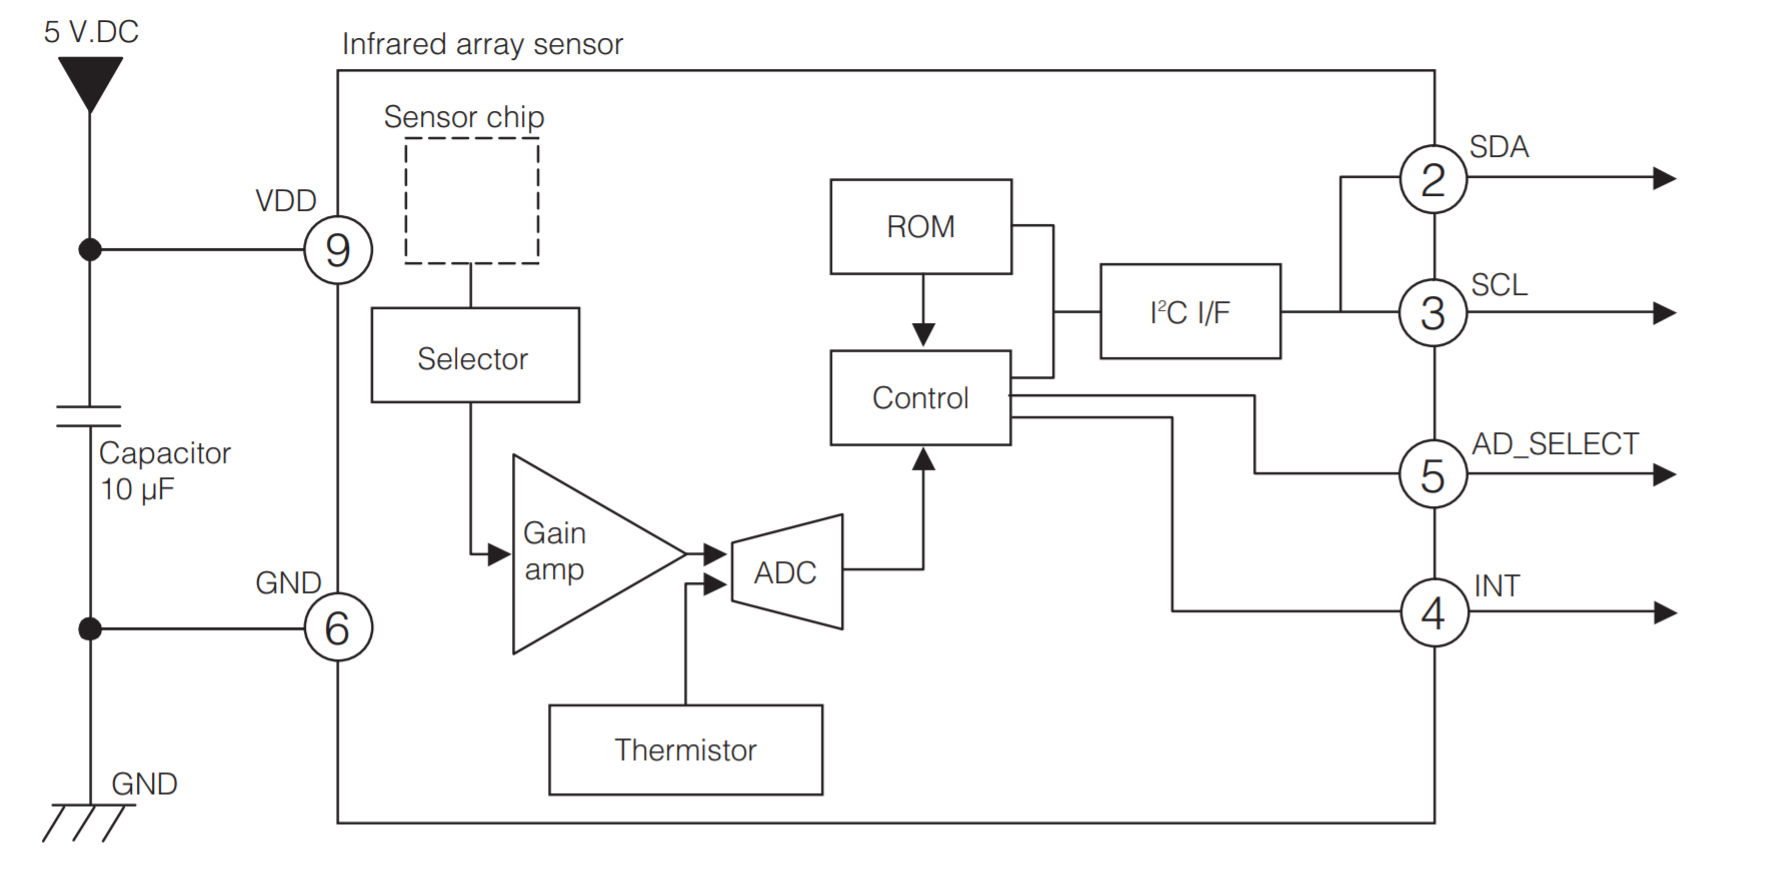
\includegraphics[width=0.8\textwidth]
	{fig/Circuit_AMG8834.PNG}
	\caption[Schema des AMG8834 Sensors]{Schema des AMG8834 Sensors} \protect\cite{velodyne}
	\label{fig:angleVLP}
\end{figure}


\begin{figure}[H]
	\centering
	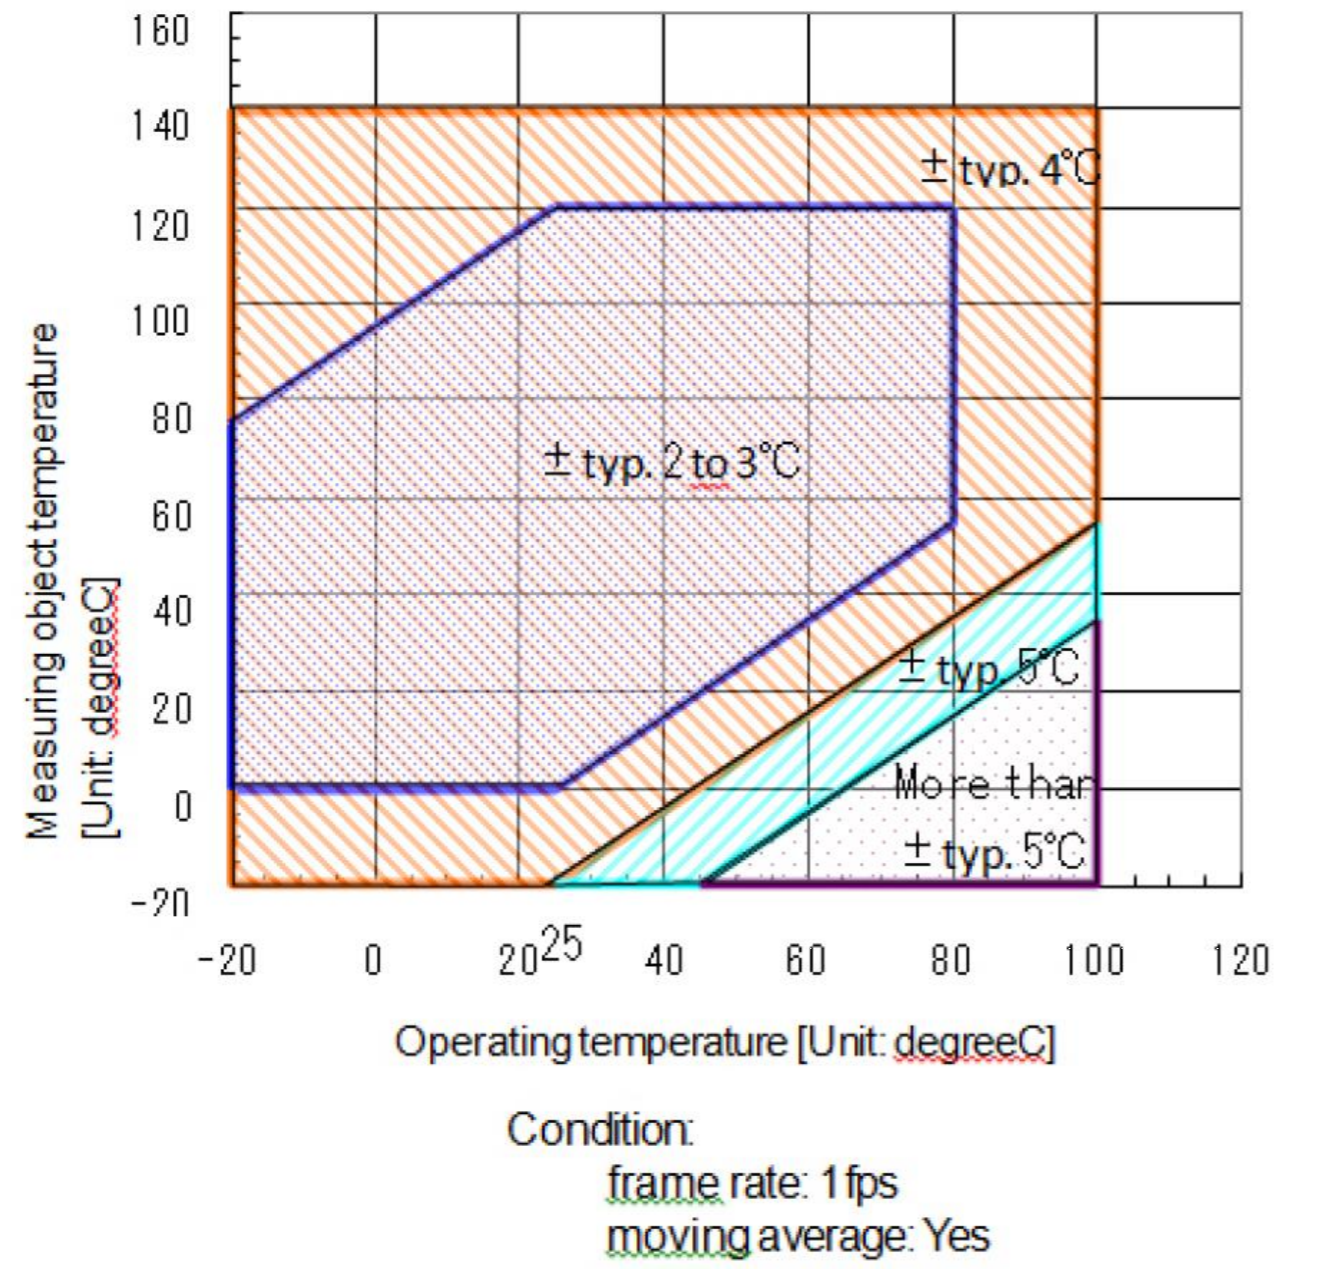
\includegraphics[width=0.8\textwidth]
	{fig/accuracy.PNG}
	\caption[Schema des AMG8834 Sensors]{Schema des AMG8834 Sensors} \protect\cite{velodyne}
	\label{fig:angleVLP}
\end{figure}
\section{zu messende Objekt}

\begin{figure}[H]
	\centering
	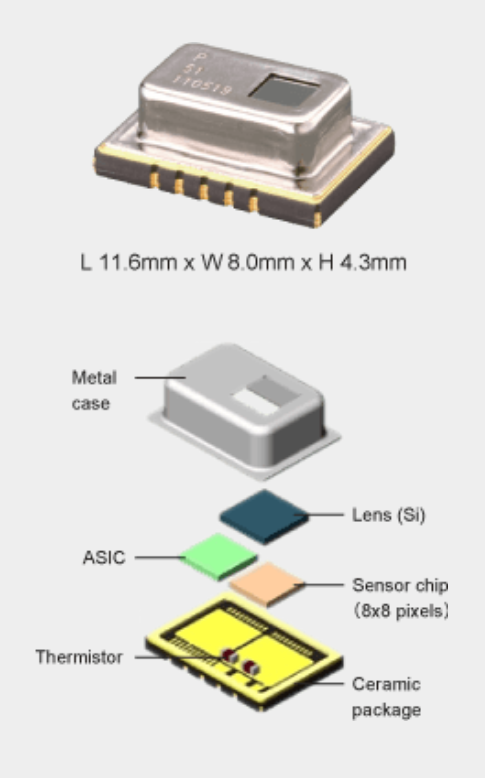
\includegraphics[width=0.5\textwidth]
	{fig/grid_eye_aufbau.PNG}
	\caption[Schema des AMG8834 Sensors]{Schema des AMG8834 Sensors} \protect\cite{velodyne}
	\label{fig:angleVLP}
\end{figure}
\section{zu messende Objekt}

\section{Störquellen}


\section{verwendete Software}